% (c) 2015 Daniele Zambelli daniele.zambelli@gmail.com
% (c) 2017 Bruno Stecca

% % \vspace{-2ex}% (c) 2012 Dimitrios Vrettos - d.vrettos@gmail.com
  \begin{center}
    \begin{hieroglyph}{\leavevmode \loneSign{\Aca GM/43/}\HinterSignsSpace
\loneSign{\Aca GM/43/}\HinterSignsSpace
\loneSign{\Aca GM/43/}\HinterSignsSpace
\Cadrat{\CadratLineI{\Aca GV/32/\hfill\Aca GV/32/\hfill\Aca GV/32/}\CadratLine{\Aca GV/32/\hfill\Aca GV/32/\hfill\Aca GV/32/}}\HinterSignsSpace
\Cadrat{\CadratLineI{{\Hsmaller\Hsmaller\Aca GV/51/}\hfill{\Hsmaller\Hsmaller\Aca GV/51/}\hfill{\Hsmaller\Hsmaller\Aca GV/51/}}\CadratLine{\Aca GV/51/\hfill\Aca GV/51/\hfill\Aca GV/51/\hfill\Aca GV/51/}}\HinterSignsSpace
\loneSign{\Aca GZ/32/}\HinterSignsSpace
\loneSign{\Aca GZ/32/}\HinterSignsSpace
\loneSign{\Aca GZ/32/}}\end{hieroglyph}
  \end{center}\vspace{-2ex}
% \begin{inaccessibleblock}
% [Immagine di una porzione dell'insieme di Mandelbrot.]
% \vspace{-2ex}
% \begin{center} 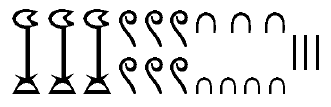
\includegraphics[scale=0.25]{img/hiero3673.png} 
% \end{center}
% \vspace{-2ex}
% \end{inaccessibleblock}

\input{\folder iperreali_gra.tex}

\chapter{Dai Naturali agli Iperreali}

\section{Dai numeri naturali ai numeri irrazionali}
\label{sec:01_introduzione}

Riprendiamo i diversi insiemi numerici che abbiamo imparato a conoscerete
mettendo in evidenza il loro ruolo come modelli per risolvere alcune classi 
di problemi e le loro caratteristiche.

\subsection{I numeri naturali $\N$}
\label{subsec:insnum_naturali}

I primi numeri che abbiamo incontrato sono i numeri naturali. Sono quelli 
che 
permettono di contare oggetti. Se sul banco ho un quaderno, una penna e un 
libro posso dire che ci sono~3 oggetti. Si può capire come il numero Zero 
abbia avuto difficoltà a farsi accettare come numero: serve per contare un 
gruppo di oggetti dove non c'è niente da contare. 
Ma ora abbiamo capito che è molto comodo considerare lo zero come un numero.
Questi numeri sono chiamati numeri \emph{naturali} 
e l'insieme di questi numeri viene indicato con~$\N$.

Nei numeri naturali sono definite l'addizione, la moltiplicazione che sono 
sempre possibili. In queste due \emph{strutture} $\tonda{\N, +}$ e 
$\tonda{\N, \times}$ valgono le proprietà: associativa, commutativa e 
l'esistenza dell'elemento neutro.

Nei numeri naturali è definita anche la \emph{potenza} ma questa operazione 
non è definita quando sia la base sia l'esponente sono uguali a zero.

Oltre a queste, sono definite anche le loro operazioni inverse: la 
sottrazione, la divisione e la radice, queste non sono definite per ogni 
coppia di numeri.

D'altra parte se su un tavolo ho~5 oggetti posso toglierne~3 e ne restano~2:
\[5-3=2\]

Ma se sul tavolo ho~3 oggetti non ha senso cercare di toglierne~5!

\subsection{I numeri interi $\Z$}
\label{subsec:insnum_interi}

I numeri possono però essere utilizzati anche come modelli di altre 
situazioni. 
Supponiamo di avere la sequenza di oggetti e di voler riferirmi ad ognuno 
con un numero che equivale al suo indirizzo o indice. In certi casi potrei 
cercare il primo elemento della sequenza e chiamarlo zero, quello che viene 
dopo lo chiamo uno e così via. Ma se ci trovassimo a lavorare principalmente 
con gli elementi compresi tra il 273° elemento e il 310° elemento, questo 
modo di fare sarebbe piuttosto scomodo. 
Molto più semplice è mettersi d'accordo di chiamare zero il 273° elemento e 
partire da lì a contarli. Ora i numeri che dovremo usare saranno quelli 
compresi tra~0 e~37. 
Ci sono inoltre delle situazioni in cui è difficile, o impossibile, 
determinare un \emph{primo} elemento della sequenza e anche in questo caso 
ci si può mettere d'accordo di assegnare ad un preciso elemento della 
sequenza il valore zero.

E chiaro che lo \emph{zero} non sarà il \emph{primo} elemento della 
sequenza, ma un valore all'interno della sequenza. Quindi è possibile 
muoversi sia sopra lo zero, sia sotto lo zero.
Per non inventare dei nomi completamente nuovi per questi nuovi 
numeri, sono stati aggiunti semplicemente due segni:~``$+$'' per i numeri 
dopo lo zero e~``$-$'' per i numeri prima dello zero. 
Questi nuovi numeri sono chiamati numeri \emph{interi} 
e l'insieme di questi numeri viene indicato con~$\Z$.

In questa situazione l'addizione può essere vista come muoversi nel verso 
di crescita dei numeri e la sottrazione come muoversi nel verso della 
decrescita dei numeri. Dato che lo zero è un elemento convenzionale non c'è 
nessun problema a togliere~5 da~3 semplicemente si arriverà nella 
posizione~2 prima dello zero detta anche~$-2$.

In questo insieme di numeri è sempre definita anche la sottrazione, anzi la 
sottrazione diventa semplicemente un caso particolare di addizione.

I numeri interi permettono di risolvere sempre equazioni del tipo:
\[x+a=0\]

Il sottoinsieme di \(\Z\) formato dallo zero e da tutti i numeri positivi
si comporta esattamente come l'insieme dei numeri Naturali. Diremo che 
questo sottoinsieme è isomorfo all'insieme~\(\N\) 
e questo ci permette di di usare indifferentemente \(+7\) o \(7\) 
senza dover precisare che \(+7\) è un elemento di \(\Z\) 
mentre \(7\) è un elemento di \(\N\).

Anche questi numeri però non riescono a realizzare un modello in certe 
situazioni che invece nella pratica si possono risolvere facilmente con un 
po' di creatività. Ad esempio come possiamo dividere~3 uova, in parti 
uguali, tra~4 persone?

\subsection{I numeri razionali $\Q$}
\label{subsec:insnum_razionali}

Con le tre uova faccio una frittata che divido facilmente in~4 parti 
uguali. 
Possiamo costruire dei numeri che permettano di calcolare sempre il 
quoziente esatto di due numeri naturali anche quando la divisione tra i due 
dà un resto diverso da zero. 
Questi nuovi numeri sono chiamati numeri \emph{razionali} 
e l'insieme di questi numeri viene indicato con~$\Q$.

Mentre nei naturali e negli interi ad ogni numero corrisponde un 
\emph{nome} ben preciso, nei razionali lo stesso numero può essere indicato 
con molti nomi diversi. 
Ad esempio il numero che si ottiene dividendo~1 in due parti 
uguali può essere indicato in in uno di questi modi:
\[\frac{1}{2}=\frac{3}{6}=\dots=\frac{45}{90}=\frac{132}{264}=\dots=0,5\]

Ogni numero razionale può essere rappresentato con un numero con la virgola 
o con una qualunque delle infinite frazioni equivalenti.

Con i numeri razionali si può sempre calcolare il risultato della divisione 
tra due numeri (naturali, interi o razionali) tranne il caso particolare in 
cui il divisore sia uguale a zero. 
In questo caso la divisione non può essere eseguita.

I numeri razionali permettono di risolvere sempre equazioni del tipo:
\[ax+b=0 \quad \text{ con } \quad a \neq 0\]

I razionali hanno una caratteristica particolare che non avevano né i 
naturali né gli interi: formano un insieme \emph{denso} cioè tra due numeri 
razionali, per quanto vicini, se ne può trovare sempre almeno un altro.

Anche tra i razionali si può trovare un sottoinsieme isomorfo all'insieme 
degli interi, cioè che si comporta come l'insieme degli interi: è il 
sottoinsieme dei numeri che, scritti sotto forma di frazioni hanno come 
numeratore un multiplo del denominatore o che, ridotte ai minimi termini, 
hanno per denominatore uno. 
Questo fatto ci permette di poter scrivere:~\(-\dfrac{7}{1} = -7\) 
senza dover precisare che il primo numero appartiene a \(\Q\) e il secondo 
a \(Z\).

Ma ci sono ancora situazioni in cui i numeri razionali non permettono di 
risolvere problemi relativamente semplici da risolvere praticamente. 
Ad esempio è stato dimostrato (già qualche millennio fa) che se il lato di 
un quadrato è un numero razionale allora la sua diagonale non lo è. 

\subsection{I numeri reali $\R$}
\label{subsec:insnum_reali}

Se prendiamo un quadrato di lato~1, la sua diagonale, per il teorema di 
Pitagora, risulta lunga~$\sqrt{2}$. 
La radice di~2 è quel numero che elevato alla seconda dà come risultato~2.
Ebbene, è stato dimostrato che nessun numero razionale moltiplicato per se 
stesso dà come risultato~2. 
Quindi, o dà un numero più piccolo o un numero più grande.

Possiamo quindi costruire due sottoinsiemi dell'insieme $\Q$ in modo da 
mettere in uno tutti i numeri minori di un certo valore e nell'altro tutti 
i 
numeri maggiori o uguali a quel valore. Nel caso della radice di~2:

\begin{center}
 \begin{tabular}{ll}
\toprule
Valore per difetto di $\sqrt{2}$ &Valore per eccesso di $\sqrt{2}$ \\
\midrule
1& 2\\
1,4& 1,5 \\
1,41& 1,42\\
1,414& 1,415\\
1,4142& 1,4143\\
\ldots& \ldots\\
\bottomrule
\end{tabular}
\end{center}

Due sottoinsiemi costruiti in questo modo si chiamano classi contigue di 
numeri razionali, cioè due sottoinsiemi di \(Q\) tali che ogni elemento 
dellprimo è minore di qualunque elemento del secondo e che nel primo 
sottoinsieme ci sono numeri che si avvicinano quanto si vuole a certi 
numeri del secondo sottoinsieme.
Due classi contigue di numeri razionali definiscono un 
numero \emph{reale} $\R$. Dato un \emph{numero qualsiasi} possiamo sempre 
realizzare due classi contigue di numeri razionali. 
Se questo \emph{numero qualsiasi} appartiene al secondo sottoinsieme è, 
evidentemente un numero razionale, se non appartiene ai due sottoinsiemi è 
un numero irrazionale. 
Ognuna di queste partizioni, dette anche sezioni di Dedekind, può essere 
considerata come un numero, cioè è possibile costruire un ordine tra le 
sezioni, sommarle, moltiplicarle, \dots

I numeri reali formano un insieme \emph{ordinato}, \emph{denso} ma anche 
\emph{completo} cioè il numero individuato da una qualunque sezione di 
Dedekind è un numero reale.
Questo permette di far corrispondere ad ogni punto della \emph{retta reale} 
un numero \emph{reale} e viceversa ad ogni numero \emph{reale} un punto 
della \emph{retta reale}. 

Anche l'insieme dei Reali contiene un sottoinsieme isomorfo ai numeri 
razionali.

Bene l'insieme dei numeri reali permette di risolvere tutti i problemi che 
possiamo incontrare?
\vspace{-1em}
\begin{center} \emph{Per fortuna no!} \end{center}
\vspace{-.5em}
Ci sono tipi di problemi che non possono essere risolti con i numeri reali.
Ad esempio calcolare la radice quadrata di numeri negativi. 
Anche questo all'apparenza è un problema del tutto assurdo: calcolare la 
radice quadrata di un numero equivale a trovare la lunghezza del lato di un 
quadrato di cui si conosce l'area. 

Ora, trovare un quadrato con area piccola si può fare, magari anche con 
area nulla, impegnandosi un po', ma trovare un quadrato con area negativa 
è proprio impossibile. 
Ma come abbiamo visto per i naturali ci possono essere fenomeni nei quali 
hanno senso operazioni che in altri sistemi sono insensate.

Prima di procedere con i prossimi insiemi numerici, però, riflettiamo su 
una particolare proprietà degli insiemi visti fin'ora.

\subsubsection{Il postulato di Eudosso-Archimede}

Proviamo a fare un \emph{semplice} esperimento mentale. Prendo un foglio di 
carta e lo piego su se stesso un po' di volte. Che spessore raggiungo?
Per semplificarci i calcoli supponiamo che il foglio di carta abbia lo 
spessore di $0,1mm = 0,0001m = 10^{-4}m$. 
Che spessore otterrò piegando il foglio su se stesso~64 volte?

Il calcolo è abbastanza semplice:

\begin{center}
 \begin{tabular}{ccc}
\toprule
Numero piegature & spessore ottenuto & in metri\\
\midrule
0 & 1 & $10^{-4}$\\
1 & 2 & $2 \cdot 10^{-4}$\\
2 & 4 & $4 \cdot 10^{-4}$\\
3 & 8 & $8 \cdot 10^{-4}$\\
4 & 16 & $1,6 \cdot 10^{-3}$\\
5 & 32 & $3,2 \cdot 10^{-3}$\\
6 & 64 & $6,4 \cdot 10^{-3}$\\
7 & 128 & $1,28 \cdot 10^{-2}$\\
\ldots& \ldots\\
n & $2^n$ & \ldots\\
\bottomrule
\end{tabular}
\end{center}

Quindi piegando il foglio 64 volte ottengo uno spessore che è $2^{64}$ 
volte lo spessore di partenza quindi basta calcolare:
\[2^{64} = 18.446.744.073.709.551.616\]
che convertito in metri dà: $1.844.674.407.370.955m$ circa che è uno 
spessore considerevole, quasi duemila volte la distanza 
Terra-Sole:~$149.600.000.000m$.

Si fa risalire ai matematici Eudosso e Archimede l'osservazione che per 
quanto piccolo si prenda un numero (ad esempio lo spessore di un foglio di 
carta), basta moltiplicarlo per un numero sufficientemente 
grande~($2^{64}$) 
per farlo diventare maggiore di qualsiasi numero (ad esempio la distanza 
Terra-Sole).

\begin{postulato}[Eudosso-Archimede]
Dati due numeri positivi \(a, b\) si può sempre trovare un 
multiplo del più piccolo che sia maggiore del più grande:
\[\forall a, b \in \R \quad \exists n \in \N \quad | \quad na>b\]
\end{postulato}

Vale anche il contrario: per quanto grande sia un numero posso dividerlo 
per un numero abbastanza grande da farlo diventare più piccolo di un 
qualunque numero.

Ma questa osservazione di Eudosso-Archimede non è un teorema, non è 
un'osservazione dimostrata, è un postulato, un accordo fatto tra matematici 
che può essere utile in moltissimi casi e che vale per tutti gli insiemi 
numerici visti fin'ora. 
Ma cosa succede se ci accordiamo che \emph{non} valga il postulato di 
Eudosso-Archimede?

\subsection{I numeri complessi $\C$}
\label{subsec:insnum_complessi}

Riprendiamo il problema della radice di numeri negativi. Si può ampliare 
l'insieme dei numeri reali aggiungendo i numeri che sono le 
radici di tutti i numeri anche di quelli negativi. Per fare ciò si devono 
aggiungere molti altri numeri (infiniti) tutti questi nuovi numeri sono 
stati chiamati numeri \emph{immaginari} che combinati con i numeri reali 
formano l'insieme dei numeri \emph{complessi} insieme che viene indicato 
con 
$\C$. 
Anche per i numeri complessi tutti gli infiniti nuovi numeri si ottengono 
con la semplice aggiunta di un solo nuovo numero: \emph{l'unità 
immaginaria} indicato con il simbolo \(i\) o con il simbolo \(j\).
\begin{definizione}
 L'\textbf{unità immaginaria} è quel numero che elevato alla seconda dà 
come risultato \(-1\):
\[i^2 = -1\]
\end{definizione}

Questi numeri hanno molte applicazioni tecniche, ma risultano anche 
affascinanti da un punto di vista estetico. La ripetizione di un paio di 
calcoli aritmetici tra numeri complessi produce il sorprendente insieme di 
Mandelbrot.

\begin{wrapfloat}{figure}{r}{0pt}
\begin{inaccessibleblock}
[Immagine di una porzione dell'insieme di Mandelbrot.]

\includegraphics[scale=0.30]{img/fractal.jpg}
\end{inaccessibleblock}
\caption{Porzione dell'insieme di Mandelbrot.}
\label{fig:mandelbrot}
\end{wrapfloat}
Ma dato che l'insieme dei reali oltre che essere un campo ordinato è anche 
completo, non è possibile aggiungere elementi ai reali senza perdere 
qualche proprietà dell'insieme numerico. 
Nel caso dei complessi l'insieme ottenuto non è totalmente ordinato.

Inutile dire che possiamo prendere un sottoinsieme dei Complessi che sia 
isomorfo ai Reali.

% \vspace{24pt}

\input{\folder iperreali.tex}




































